% !TeX root = ../main.tex
\chapter{Introduction}\label{chapter:introduction}
Autonomous driving has attracted a great deal of attention either in research organizations or in industry. In recent years, important car manufactures all over the world have invested lots of money to produce semi-automatic or even full-automatic vehicles. Among many of the autonomous driving areas that researchers has been working in these days, \acrfull{ap} is one of the oldest subject in autonomous driving. One of the first idea for car parking was proposed  in 1934 \cite{firsParking}. However, this research did not lead to a produced vehicle. One of the successful \acrshort{ap} project presented by the researchers from (\acrfull{inria}) in mid of 1990. They applied this method on an electric car called Ligier \cite{parkingManeuver}. Many researchers impressed by their algorithm and new algorithms has been published based on this method i.e, \cite{twoCircles}. However, most of the parking algorithms has been proposed theoretically and not all of them practically used for parking. Among companies who applied \acrlong{ap} in their produced cars, we can point to Toyota, Ford, Lincoln, Jeep,Volkswagen, BMW, Mercedes-Benz and AUDI. However, their systems still depends on human and accelerating/braking inputs are not fully automated. Bosch company has recently planed to produce a fully automated parking system which allows the driver to leave the car and activate parking from his smartphone \cite{usConference}. Apart from the commercial issues and the fact that most of these companies should adapt to new technologies to survive beside their competitors, what are the benefits of \acrshort{adas} and \acrshort{ap} for drivers or in general for passengers? One of the arguments of making \acrfull{av} is to save the fuels because most of the \acrshort{av}s are powered by electricity instead of gasoline \cite{otherThesis}. Other studies shows that most of the accidents are because of human's error like driver's inattention, distraction, stress or tiredness. In particular, \acrshort{ap} could help drivers to find parking spots easily because drivers do not have a wide view of the parking or maybe there are parking spots which are not obvious because either they are far from the driver or they are hidden by other cars or objects \cite{detection-with-CNN}. \acrshort{ap} offers more efficient parking by reducing waiting time of passengers to search for parking spot. After they arrive to the destination they could just drop by and vehicle will search for a parking place by itself. \\
Autonomous parking consists of two main problems: detection and maneuver. Many researches has been done in both areas as will be described in details in the next chapter \ref{chapter:related_wrok}. The methods have been defined for detection phase, are either based on sensors or visual features. Hence, detection phase itself can be categorized into 2 groups: free-space-based and parking-slot-marking-based methods \cite{markingPointConf}. Free-spaced-base methods use sensors to find a free space between adjacent vehicle and most of them use UltraSonic sensors. Parking-slot-marking-based methods tries to use visual features like line markers from the parking lot which is also called marking points. In maneuver step the problem is to find a perfect algorithm to control maneuvering of the vehicle to detect parking lot. Many researches have been also devoted to this area. Most of the parking maneuver algorithms are based on these two methods: tracking and posture stabilization \cite{fuzzy}. The idea of first method is to design a control path in which an actor (Robot or vehicle) should follow this path as a reference trajectory. Second one tries to stabilize the position of the actor to a desired final posture. This thesis presents a research on whole parking process from detection phase to maneuver phase and specifically considers parallel parking implementation. 
\section{Motivation and Problem Statement}
Although many approaches have been presented on \acrshort{ap} but most of the methods are designed for a robot or what is called \acrfull{clmr} like \cite{fuzzy} or \cite{twoCircles}. However, there are less methods which specifically designed for a real vehicle so this field is still open for new research either to complete last methods or to make them practical on a real car. In addition, most of the recent methods like \cite{novel-CLMR} and \cite{visual-parking-slot} are designed for garage-based parking which is mostly based on the vertical or diagonal movement of vehicle(\ref{concepts}) so fewer methods considered parallel parking. However, it seems that automation of parallel parking is more necessary because parking on streets is more difficult than a parking-lot as it is more difficult to find a parking place on the street where there is more traffic and also more barriers to prevent parking there and the probability of human's errors on street parking are more than parking in garage. Besides, for parking on street(or parallel parking) many thing should be considered to prevent accidents. In garage parking, parking places are clear and there is less traffic(from people or cars) there and even sometimes there are helpers in garage to guide the drivers.\\
This thesis implements a simulation of parallel parking using a new simulator called Carla. Implementation includes a complete parking process from the the detection of parking place to control the vehicle movement to the parking lot. Python will be used as \acrshort{api} which is directly connected to Carla and for the detection part, Matlab tools has been used. This implementation is a Combination of visual-based and sensor-based methods. In detection part, camera sensor is used to provide visual data for vehicle detection and to make a perfect maneuver algorithm which protected vehicle from crashes, sensors are applied to detect obstacles and make range measurements. 
\section{overview}
According to the above descriptions, diagram \ref{fig:sysreview} illustrates an overview of this thesis.
Chapter \ref{chapter:Background} presents a background and fundamental knowledge which is required to follow this work. Chapter \ref{chapter:related_wrok}, describes related works and methods that presented in visual-based as well as sensor-based parking detection and also various parking-path methods. Detail explanation of each step of thesis which has been seen in flowchart \ref{fig:sysreview} can be found from Chapter \ref{chapter:Parking Space Detection} to Chapter \ref{chapter:Parking Maneuver}. Chapter \ref{chapter:Implementation} illustrates the implementation of each step and all of the challenges during implementation phase. Chapter \ref{chapter:Evaluation} provides an Evaluation of the implemented steps and considers how well are the simulation results. Chapter \ref{chapter:limitations} says about limitations and problems during this work. Chapter \ref{chapter: future_works}, gives an outlook on possible future developments and finally Chapter \ref{chapter:Conclusion} summarizes this thesis.

\begin{figure}
\centering
     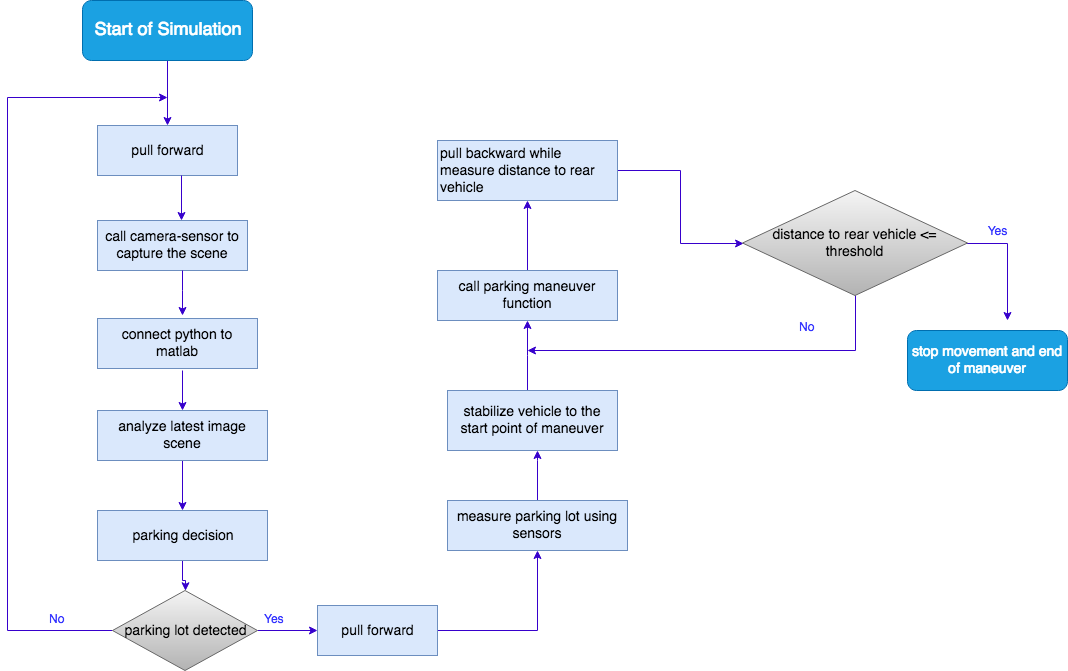
\includegraphics[width=14cm]{images/system.png} 
     \caption{System Review}
     \label{fig:sysreview}
\end{figure}